%!TEX root = ../dissertation.tex
\section{Obsolete Stuff}

%Popek and Goldberg~\cite{Popek1974-xx} identified three properties that a virtualization system must guarantee:
%\emph{efficiency}, \emph{resource control}, and \emph{equivalence}.
% \cjr{I'm going to talk about interposition, compatibility, and isolation below. I'd like someone to go look at the popek and goldberg paper, cite it, and try to generate an argument about why we care about this list, and not the list from that paper.}
% \aak{I looked up the original paper... It mostly talks about virtualizability of an ISA, which is orthogonal to our concerns, but the 3 properties they highlight actually are relevant to us.... Interposition and isolation (our terms) essentially fall into the safety category. Compatibility is fidelity + engineering effort.}
%%%%%
%% Bugnion, Neih, and Tsafrir
%% defined virtualization as ``the application of the layering principle through enforced modularity
%% whereby the exposed virtual resource is identical to the underlying physical resource being
%% virtualized''~\cite{bugnion_neih_tsafrir}\hyu{Do we really need this quote?}.


%%%%%%%%%%%%%%
%% STACK DIFF
%%%%%%%%%%%%%%

\begin{comment}
\begin{figure}[!t]
	\centering
	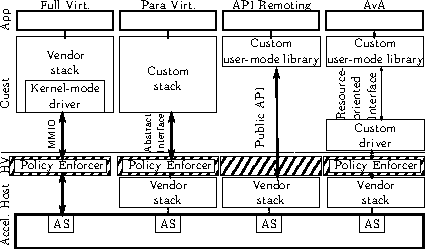
\includegraphics[width=\linewidth]{images/stack_diff.pdf}
	\caption{Different stack designs. HV = Hypervisor. TODO: fix lines (size and pattern); align all the elements of the drawing as needed; Make hatching lighter; split accelerator into separate blocks like the app; general clean ups.
    \cjr{This is a pretty good, not sure it's completely there yet. It does capture the key differences
    if you already happen to know what they are. Why is our resource-oriented interface a box? Components
    have interfaces, but an interface is not a component.
    Maybe the striped boxes that represent hypervisor interposition should be represented by the kind of
    line? An interposable line looks (dramatically) different from a non-interposable one? A more
    traditional way to show it would be to enclose parts that are in a hypervisor in the hypervisor.
    What's the one with the abstract interface? I think we should go one more round of revision to see if we
    can make this work, but it's not completely working in its current state.}
  \amp{I took a crack at this. Any thought are appreciated. I have \emph{not} tried to make it look nice. Just think of this as a mock-up. I'll clean up all the arrow heads and stuff if we decide to use it.}
  \cjr{AMP: great stab. Issues: 1) What is and isn't in the hypervisor? 2) When is and isn't there a virtual device? 3) What is a resource-oriented interface? We've been using the term, but I still don't really know what it means. Is it a BAR? A ring in a BAR?
    4) What's an AS? 5) Should the arrow in API remoting have a curve that jumps over the hypervisor? 6) Why isn't htere anything special in the hypervisor or above the vendor stack in the AvA case?}
	}
	\label{fig:stack_diff}
\end{figure}
\end{comment}

%In order to address this situation, we must first understand how it arose: in this section, we look at the \emph{siloization} of %accelerator software stacks, and how this makes traditional accelerator virtualization mechanisms inviable.
% To explain why the other virtualization techniques are not selected,
% this section considers related work for virtualization of compute/offload accelerators
% and summarizes limitations of existing virtualization techniques when applied to accelerator silos.

%Accelerators are purpose-built processors, specialized for specific tasks.
% more efficiently than general-purpose processors.
%Accelerator hardware interfaces represent a peculiar \emph{duality}: their control mechanisms are similar to those of I/O devices, while %they are primarily compute devices.
%This \emph{duality} has given rise to a interesting challenge for virtualization:

%\cjr{Does this head off reviewer E? (see below) I think it does.}
%\reviewer{E}{A central premise of this paper is that accelerators will not provide support for virtualization (\S\ref{s:bg_tech}). There are two problems with this premise. First, it runs counter to trends in processor and traditional I/O devices, all of which have added support for virtualization. Second, it is contrary to to AvA's own assumption, which is that all accelerators will provide process-level isolation (a form of virtualization!) to enforce memory isolation, as GPUs do today. Without process-level isolation, AvA runs requests from only one VM at a time, and even this isn't sufficient -- AvA should really make sure that only one VM's data set is in memory at a time.}

%within the software \emph{silo} are impractical: they either require reverse-engineering proprietary interfaces (as in the case of the VMware SVGA vGPU), or result in severe overheads that invalidate the performance gains that makes acceleration appealing in the first place~\cite{gpuvm}.
%We observe that any virtualization technique that \emph{breaks the accelerator silo} has significant drawbacks:
% which have collectively prevented the emergence of production accelerator virtualization software:


%\reviewer{B}{This paper argues that it is difficult for a para-virtualized device to support interfaces required by multiple GPU programming frameworks. However, the para-virtualized device only needs to provide the same interface as one real hardware, which is enough for different frameworks.}\cjr{I'm not sure what to do about this idiot. We've said multiple times above that there are different hardware interfaces. This may be a lost cause. }

%\reviewer{A}{Please include a list of contributions.}

%\reviewer{D}{POST-REBUTTAL FEEDBACK/ELABORATION: Thanks for the response. I decide to lower my score from ``Accept'' to ``Weak accept'' after reading the response and the other reviews.
%	The main reason is that I'm not able to articulate the contributions to champion the paper. The paper is an interesting read and the work is solid. So I still stand at the positive side.
%	The response does not address my concerns about CAvA. I still don’t really understand how the code generation works.}
%https://github.com/ava-virt.\hyu{Looks we don't really need this sample repo in the paper. And I want to show the repo name ``ava-virt/sample'' to indicate that it's anonymous.}
%\reviewer{C}{What are all the advanced virtualization features? Or live migration is the only one? It will be good if you can call the other features explicitly, e.g., ``AvA supports advanced virtualization features include live migration, A, B, and C.''}

\reviewer{E}{It would help to get a little more background on API forwarding/remoting (Section \ref{s:bg_api_remoting}). Does the user-level computing framework issue the request to the accelerator, and if so, what interface does it use? The API server appears in Figure \ref{fig:high_level_design} but not in Figure \ref{fig:silo}.}
\cjr{I think we've dealt with this as much as possible}




%Another side effect is the absence of the throughput control among VMs,
%because the GPU scheduler slices the cycles according to the application number--%
%one VM can run massive number of applications to DoS the applications from other VMs.
Separate scheduling policies in the hypervisor and hardware require coordination.
Hypervisors (e.g. VMware ESX and Linux KVM) controls the VMs' priority by changing their vCPUs' priority.\cjr{not sure where this was going, so not deleting yet.}

\reviewer{C}{The paper is hard to follow and not well written. A lot of Section 4 needs more discussion (e.g., justification of why the choice of the design). I'm not sure if I fully get the motivation of your core design of having separate API Server processes to execute exported APIs. Why can't the interposed APIs be executed within the VM itself? Aren't the VMs already isolated? Is it because the accelerator Silo is hard to be virtualized? Or am I missing something because I don't fully understand your writing?}


% \cjr{Should we observe this is the only functionality you get out of GRID and BitFusion?}
% \cjr{We don't claim to handle device-side malloc/new do we? It's probably not a problem since there is a heap size set at e.g. cudaInitialize.}
% \hyu{I like the old way to introduce the memory partitioning feature. At least it should be in a separate paragraph. If your concern is that we don't ``actually'' implement it, we can support it once we submit the paper. I'm 120\% sure it's a really easy piece of work.}

%\hyu{And we currently don't have a section introducing how we track the memory resource usage (it's reported by \worker and also checked by router from API semantics). I guess you imply that the shared resource in the %first sentence also includes the device memory, but the memory resource management is not handled by ``rate limiting''.}
%\aak{better?}
%\hyu{perfect.}
% The router flags all API invocations that would exceed the guest's memory
% when it receives the flagged invocation.

\begin{comment}
\aak{cut out speculation}
For finer-grained accounting, \AvA can be extended to leverage existing
profiler APIs (e.g., Tensorflow Timeline and CUDA Profiling Tools). The memory
profiling and \worker behavior can both be specified in the specification.
\end{comment}

% The accuracy of the approximation will affect the level of fairness \AvA can provide.
% In \AvA, the resource usage is reported by the \worker to the hypervisor \emph{before} or \emph{after} an invocation is finished, and the report point is determined in the specification.
% \AvA also allows to estimate the resource usage of an invocation before it is received by the worker.

% For example, the code may estimate the bus bandwidth used by a data copy call by simply using the number of bytes copied.
% The worker reports the used bus bandwidth to the hypervisor and hypervisor control the API rates from VMs to limit the bus usage via the same interfaces in the fair scheduling scenario.

\begin{comment}
The router can also be augmented with policies expressed in a restricted
language like eBPF~\cite{ebpf} in order to support arbitrary scheduling
policies. Neither of these are implemented in our prototype.
\aak{dropped for being too speculative.}
However, \AvA can use the profiling interface of the API for more precise measurements (such as \lstinline|clGetEvent|\-\lstinline|ProfilingInfo|).
We conjecture that these approximations will provide a useful level of performance isolation, despite their inaccuracy.
\end{comment}

\reviewer{B}{In Section 6.4, AvA controls the device utilization time of each VM. How to calculate the usage time of a VM? AvA only allows the hypervisor to hook public APIs. If a VM invokes an asynchronous API to run an application on GPU. How does the hypervisor calculate its execution time?}
\hyu{He points to a wrong section.}

\begin{comment}
\paragraphbe{Manager} is part of the \AvA core, and runs as a privileged process in the host,
tracking creation and destruction of VMs and guest applications. When a new application starts,
the manager chooses a \worker from the \textit{\worker pool} to service the application.
\aak{We don't talk about the manager, around here, in these parts. It decided to join the implementation.}
\end{comment}

% contexts.
% This ensures that failures resulting from an invocation are isolated from other \workers and guest applications.

% \AvA protects the system from potential denial-of-service and information leakage.\aak{Whoever wrote this, please explain how.}

 % because those can be modified by the VM administrator to behave maliciously.
\begin{comment}
As the \worker executes a rich set of commands from the guest application, it
exposes a very large surface for an attacker to exploit.
As a protection, all API calls in \AvA must be mediated by the router to be
verified, at the cost of communication latency.
\aak{I've commented this out because we don't implement this, and I don't feel we have anything particularly intelligent to say.}
\end{comment}


\begin{comment}
\begin{figure}[!t]
	\centering
	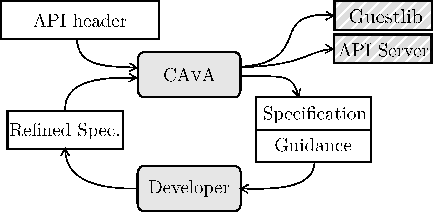
\includegraphics[width=.8\columnwidth]{images/work_flow.pdf}
	\caption{\AvA virtualization workflow. Rounded boxes represent actors, and squared boxes represent input and output. API-specific components generated by \CAvA have shaded backgrounds to maintains visual continuity with Figure~\ref{fig:high_level_design}.}
	\label{fig:dev_flow}
\end{figure}
\end{comment}

% The common API-agnostic transport infrastructure further enables a number of
% optimization opportunities that generalize across accelerator stacks
% (\S\ref{s:impl}).

% \CAvA generates the API-specific components
% (i.e., guest framework libraries, and the \worker) of the virtualization stack
% from a specification describing the accelerator's APIs.
% The guest libraries and driver communicate with the \worker component through
% the \AvA router, which runs in the hypervisor.

% The API-agnostic components of \AvA (the \emph{guest driver}, an \emph{
% \vdev}, and a \emph{router}) implement internal
% functionality.%The flexibility and modularization enables \AvA's components to be distributed so as to support hardware resource disaggregation,
%for example \AvA is compatible with disaggregated systems such as LegoOS~\cite{legoos}.


\begin{comment}
\begin{figure}[t!]
	\centering
	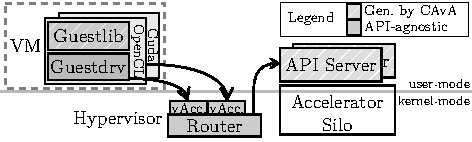
\includegraphics[width=\columnwidth]{images/design_high_level.pdf}
	\caption{Overview of \AvA. The accelerator silo is detailed in Figure~\ref{fig:silo}. Components with striped backgrounds are generated from an API specification. Components with solid backgrounds are API-agnostic.
		\reviewer{B}{In Section 4.2, this paper mentions that "AvA�s API-agnostic components (router, \vdev, and guest driver) must be implemented by each hypervisor". Meanwhile, as shown in Figure 3, for each accelerator API, the hypervisor developer needs to implement a \vdev and multiple versions of guest drivers for multiple supported guest OSes. It seems that such work cannot be performed automatically. How much developing effort is required to implement these components? I would like to see more discussion on these.}
		\hyu{We forgot to mention that the separate drivers are for security in \S\ref{sub:components}.}
		\reviewer{F}{there's a mismatch between labels in Fig 3 and the discussion, e.g. where are the ``vendor drivers'' in the fig? Abbreviations must be defined. It took me a while to realise that what looked like the puzzling ``vAccIvAcc'' was in fact two separate boxes with ``vAcc''.}
	}
	\label{fig:high_level_design}
\end{figure}
\end{comment}

\begin{comment}
\begin{figure*}[!!thp!]
	\centering
	\begin{minipage}[t]{.5\textwidth}
		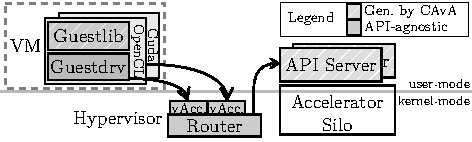
\includegraphics[width=\columnwidth]{images/design_high_level.pdf}
		\caption{Overview of \AvA. The accelerator silo is detailed in Figure~\ref{fig:silo}. Components with striped backgrounds are generated from an API specification. Components with solid backgrounds are API-agnostic.
		\hyu{The user-kernel boundary may not be correct if we include some user-space service into hypervisor; vAcc might be drawn larger, and I think it should cross the boundary.}
		}
		\label{fig:high_level_design}
	\end{minipage}
	\qquad
	\begin{minipage}[t]{.85\columnwidth}
	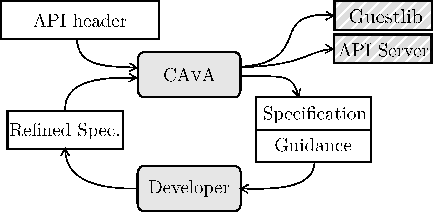
\includegraphics[width=\columnwidth]{images/work_flow.pdf}
	\caption{\AvA virtualization workflow. Rounded boxes represent actors, squared boxes represent input and output.}
	\label{fig:dev_flow}
	\end{minipage}
\end{figure*}
\end{comment}

\reviewer{E}{To smooth the use of different accelerators with different interfaces, AvA uses the time-honored technique of proposes a new standard, which in this case is a new para-virtual device for transport.}%
\hyu{I might put this review in the wrong place.}%
\cjr{This was never a critique to begin with.}%

% Custom scheduling policies are expressed in the specification usingm
% eBPF~\cite{ebpf}~\cjr{OK?}, and dynamically loaded into the router as needed.
\reviewer{E}{I'm not sure how serious a deficiency it is not to provide language-level safety guarantees (Section 4.1) for the code running in the Router module. Is this referring only to the policy code that's running in the Router module (in which case it's not a serious deficiency), or is it also referring to the requests themselves (in which case it is a serious deficiency)?}
\cjr{I think we've dispatched this by using BPF}
% Our current prototype provides flexible policy but does not yet provide language level safety guarantees.


% \hyu{This sentence is incorrect, the mediated virtio-vsock channel doesn't use this abstraction. Instead, we built a vsock channel on top of virtio-sock for transport and mediation; we built a shm channel on top of virtio-vsock and shm for transport and mediation. That's to say the abstract interface is higher-level than the virtio-vsock channel. I might give the ``vsock channel'' a confusing name. But I do think we should say sth. about mediation here.},
% Commands include ,
% so there may well be more commands than API functions.
% \cjr{I don't see how this description of a general channel fits with vsock-virtio. WTF?}
% \aak{I moved virtio-vsock to implementation, where it belongs. This section shouldn't be talking about vsock or SHM. Too low-level...}

%~\cjr{say something about handling in-memory state?}
%\amp{Addressed?}
%\cjr{yes. thanks.}
% across protection domains.
%We have not yet implemented this feature in \impl.
%\cjr{This caveat should come out in impl, not here, if it comes out at all. We've built and measured this feature, just not in the current version.
%Consequently, I think we've learned enough about it to talk about it.}

\reviewer{A}{What is the performance of process-level isolation? Is it sufficient to share between VMs?}

\reviewer{B}{This paper mentioned that AvA re-purposes process-level isolation provided by the accelerator silo to support cross-guest and cross-process isolation. However, existing accelerator vendors (e.g., NVIDIA) provide two methods to allow multiple processes to share the same GPU. The first one is time sharing which only one process can access the GPU at one time. The second one is compiling all processes' code to one kernel and running them concurrently in the GPU. There is no isolation between the code from different processes. Which method is used by AvA? The previous one may cause resource waste and the latter has no isolation. How AvA addresses this issue?}

\reviewer{C}{Another main question I have is how you isolate and protect resources in accelerators themselves. Or are you assuming another system to handle this? When I read the title, I thought that's what ``virtualizing accelerators'' mean.} \hyu{The understanding of ``virtualization''.}

\reviewer{E}{Since memory isolation is the main type of low-level isolation required, the only aspect left for AvA to isolate are the high-level policies. AvA's Router module monitors the resources (processing time and memory allocation) based on the explicit semantics of the requests, and enforces scheduling policies based on its understanding and perhaps measurements of these requests.}

% \AvA supports throttling the API requests as the Google Compute Engine API rate limits~\cite{gce-rate-limits} and AWS API throttling~\cite{aws-api-throttle} to protect the \AvA components (such as router and \worker) and physical resources from bursting requests.
% Unlike Google Cloud, \AvA delays the application's API requests rather than throwing \texttt{rateLimitExceeded} error when it exceeds the pre-configured hard threshold.
% The type and cost (of tokens) of APIs can be annotated in the specification.
% By mediating the transport layer, the hypervisor is able to provide 6 interposition points to enforce various resource policies: VM start and destroy, guest application start and termination, API invocation request and response.
% Forwarding the API calls through the hypervisor gives it a view into device utilization.


\reviewer{D}{\S\ref{s:compiler} (CAvA) is a typical example. I can’t understand how CAvA works based on the writings of S5. Given that half of the components are auto-generated by CAvA, I expect a clear description on how CAvA generates the code and the analysis of the correctness and effectiveness of the generated code. However, Section 5 is very procedural and starts with a large number of syntax details, without giving a high-level overview. Specifically, \S\ref{s:code_gen} (Code Generation) is merely an explanation of three examples rather than an explanation of code generation.}

\reviewer{D}{I would urge the authors to carefully write the middle sections if the paper gets accepted. Specifically, the writing should help readers catch background and grasp the high-level ideas. Examples (e.g., Figure 6-8) should only be used to help demonstrate the explanation of the design and implementation -- you can’t expect the readers to understand the ideas and mechanisms by reading a few code examples.}

\reviewer{D}{I also do not understand how the three code snippets connected. In Figure~\ref{fig:worker_code_template}, you refers to ``argument processing as Figure~\ref{fig:guest_code_handler_template}'', what exactly is the argument processing part in Figure~\ref{fig:guest_code_handler_template}? One thing you can do is to use figures to illustrate the semantics of the code blocks.}

\begin{comment}

Some synchronous APIs may safely be executed asynchronously
Asynchronous functions return immediately after the call command is sent in \AvA.
We leverage this to our advantage:
% The developer will generally annotate functions that are asynchronous in the original API, however this is not required.
For example, \lstinline|clSetKernelArg| is a synchronous OpenCL API,
but can be forwarded asynchronously to reduce the overhead of these calls at the cost of fidelity:
asynchronous calls are only semantically correct when the call has no output of any kind, meaning asynchronous calls cannot report errors faithfully.
In most cases, the error can be delivered from a later API call, but this will not be faithful to a local execution.
% This unfaithful semantics only occurs if an error occurs, and will only affect the program execution if it handles the error differently depending on which call reports it.
Similar techniques were applied in vCUDA (lazy RPC)~\cite{vCUDA} and rCUDA (API batching)~\cite{rCUDA} with the same loss of fidelity.
%In addition to errors, asynchronous calls can support output values which are newly allocated object handles (such as \lstinline|event| in \lstinline|clEnqueueReadBuffer|).
%This technique can also support non-allocated handles at the cost of fidelity: allowing non-allocated handles makes handle equality in the guest unreliable.
\end{comment}

\reviewer{D}{the evaluation on sharing and multi-tenancy is not as solid as the other part of the evaluation. Figure 13 shows that even the native configuration of a 2-guest VMs leads to ~2X penalty compared with an unshared case (so is sharing really needed?). Basically, I’m not sure how representative your results are -- is it simulating the worst-case scenario?}


\reviewer{A}{How much of the auto-generated annotations need to be amended for the APIs in the evaluation?}

% \hyu{We don't mention \worker pool}, but the FPS drops 7.5\% on average.

% \amp{Update this paragraph once we have either measured QAT with zero-copy or decided not to do so. Microbenchmarks show that zero-copy works exactly as expected.}
% offload mode, as support for asynchronous offload in \AvA was incomplete.
% \hyu{explain synchronous vs asynchronous.}\cjr{cut or say why}\aak{say support for async is incomplete at time of submission}.
% , as discussed in \S\ref{s:breakdown}.
% To better support high-data-rate devices, \AvA must implement a zero-copy mechanism to eliminate the data transfer overheads. We plan to implement this in future work.
% The Intel QuickAssist is self-virtualizing via SR-IOV, but it supports on
% static allocation of resources and round-robin scheduling .

% the effect of API forwarding on a kernel-bypass high-throughput device.
% in a synchronous manner. The application is


\begin{comment}
% \subsubsection{Runtime Breakdown}
% \label{s:breakdown}

To characterize overhead sources and performance trade-offs in \AvA, we measured the percentage of time spent in various phases while using an \AvA virtualized accelerator.
Figure~\ref{fig:breakdown} presents the breakdown data for four benchmarks that use a different API each (OpenCL \texttt{dwt2d} on NVIDIA 1080, CUDA \texttt{gaussian} NVIDIA 1080, TensorFlow image recognition, and QuickAssist QATzip).
% For each benchmark we measure five categories of time:
% the \emph{loading} time of the \AvA guest library (\SI{3.8}{\milli\second} on average);
% the \emph{transfer} time for commands and data;
% the time spent \emph{marshaling} and \emph{unmarshalling} value into and out of the commands;
% the \emph{execution} time of the compute kernels; and
% \emph{uncounted} time, including data load and CPU computation in the application.
\aak{The data presented in the breakdown figure is hard to explain. Why is dwt2d a relatively high overhead benchmark when most of it's time is spent in execution? TF-image similarly spends a lot of its time in execution and has much lower overheads... Gaussian has almost as much data movement overheads but its RE2E is almost 1, while QATzip RE2E is 1.38...}
\hyu{CU\_gaussian breakdown is wrong--cuLaunchKernel is async, so some kernel execution time was counted into transfer. I'm going to call sync() after each cuLaunchKernel so that we can get accurate API execution time.}
% Benefit from the asynchronous APIs and multi-threaded applications,
The majority of overhead introduced by \AvA is from command and data transfer, which increases linearly with data size.
These phases can often \emph{overlap} with the execution phase, hiding the overhead of data transfer and processing.
% (see \S\ref{s:opt_eval} and Figure~\ref{fig:end2end_compare}).

\begin{figure}
	\centering
	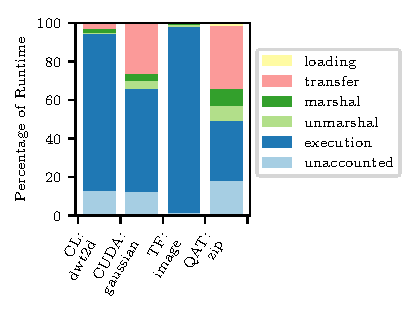
\includegraphics[width=.75\columnwidth]{data/breakdown/breakdown.pdf}%
    \vspace{-1em}
	\caption{Runtime breakdown of four different benchmarks and APIs.
	Guest library \emph{loading} includes the time of connecting to the worker.
	\emph{Transfer} time is spent transporting commands and associated data.
	\emph{Marshal} and \emph{unmarshal} time is spent putting data into and extracting data from commands.
	\emph{Execution} is the time spent on API execution in the \worker.
    The \emph{unaccounted} time is mostly data load and CPU computation in the application.}
    % Any \AvA overhead not shown was too negligible to measure.}
	\label{fig:breakdown}
\end{figure}
\end{comment}

% We think the isolation and scheduling guarantees that \AvA offers are a worthy trade-off for data-intensive applications with less extreme characteristics.
% \aak{Add text about the call intensive data if we choose to use it.}
% and the patterns can be summarized as follows:


